%!TEX root =  ../main.tex

\mychapters{Conics}{conics}{\chapdir/pics/NM_12-06-06_0576_(7175101925)}

Rotated, Eccentricity

\newpage
\chapterminitoc

\newpage
\invisiblesection{Introduction to Conics}
\marginlessinput{\chapdir/DD01p}
\newpage
%!TEX root =  ../main.tex

\subsection{3D Geometry}
For nearly 3,000 years, mathematicians have been interested in shapes called
conic sections.  Why?  What are they?  Surprisingly, they are the means to answer some
very basic problems, like doubling the size of a cube, or why it is almost impossible to make
a square with the same area as a circle.  While the Ancient Greek geometers were interested
in such problems, it is far easier to consider them in light of analytic geometry, where we 
lay down the Cartesian plane, and place shapes in it, analyzing the algebra of their equations.

\marginfig[-0.5in]{\chapdir/pics/ConicSections_ajl.png}{The conic sections.}
The problems you worked in the lab were examples of three out of the four conic sections.
Why are they called such?  It is easy to model a cone intersecting a plane.  If we
imagine the cone as an idealized version of itself, it extends both up and down, forever
in two directions.  The plane of intersection is also the infinite plane of geometry, a flat
sheet that extends forever.

If the line through the middle of the cone intersects the plane at $90^\circ$ precisely
(what mathematicians call \textbf{normal} to the plane), then the shape on the plane will
be incredibly symmetrical, a \textbf{circle}.  Any slight variance in that angle will produce a
distorted circle, what is ordinarily called an `oval', but in mathematical parlance, an
\textbf{ellipse}. If we continue to tilt the plane, the ellipse will widen and widen.  As we
achieve an angle parallel to the side of the cone, the shape is our old friend, the 
\textbf{parabola}.  Any angle past that will result in intersecting both parts of the cone,
a shape known as a \textbf{hyperbola}.

\subsection{Graphing form}
\subsubsection{Circles}
Drawing circles is very easy and so is the algebra equation underlying them.  With a center
at $(h,k)$ and radius $r$, they can be quickly graphed, even by hand.

\marginfig[-0.5in]{\chapdir/pics/Conic_sections.png}{The angle of intersection of the plane 
and the cone may be plainly seen in the projection.}
\begin{derivation}{Equation of a Circle}
\label{eq:circle}
\begin{equation}
(x-h)^2+(y-k)^2=r^2
\end{equation}
\end{derivation}

\subsubsection{Ellipses}
We could imagine an straight-forward algebra manipulation which mirrors the geometric
manipulation from circles to ellipses: begin with Eq.~\ref{eq:circle}.  Now divide both sides 
by $r^2$:
$$
\frac{(x-h)^2}{r^2} + \frac{(y-h)^2}{r^2} = 1
$$
If we consider that the two radii represented in the denominators might be different 
(perhaps we might relabel them as $r_1^2$
and $r_2^2$), then we are very close to the graphing form of the equations for ellipses, and
we have a visual parallel: an ellipse is a circle with different radii for the $x$ and $y$!

\begin{derivation}{Equations of Ellipses}
\begin{equation}
\label{eq:ellipses}
\left(\frac{x-h}{a}\right)^2 + \left(\frac{y-k}{b}\right)^2 = 1 \quad \text{or} \quad \left(\frac{x-h}{b}\right)^2 + \left(\frac{y-k}{a}\right)^2 = 1
\end{equation}
\end{derivation}
By convention, we call whichever radii is bigger $a$, hence the two different forms.  (It will become
clearer in §DD.04 why.)

\subsubsection{Parabola}
You have done a lot of work with parabolas over the years, and the vertex form of Algebra II
requires very little manipulation to adapt to our purposes here (i.e. $y=a(x-h)^2+k$).  The only
caveats are that we like to keep the unit $(y-k)$ together, and that $a$ is four times the focal
length, conventionally called $p$.  Also, there are parabolas that open up-down, as well
as those that open left-right, as we saw in §3.3

\begin{derivation}{Equations of Parabolas}
\begin{equation}
(y-k) = 4p(x-h)^2 \quad  \text{or} \quad (x-h) = 4p (y-k)^2
\end{equation}
\end{derivation}

\subsection{Hyperbolas}
\marginfig[-1in]{\chapdir/pics/Drini-conjugatehyperbolas.png}{Hyperbolas can be horizontally or vertically oriented.}
Hyperbolas are very likely the least familiar to you of any of these objects.  Of course, 
$y=\frac{1}{x}$ is a hyperbola, but that can be hard to see, unless you turn your head
$45^\circ$ to the left!  If you look at the hyperbola $x^2-y^2=1$, some of the standard 
features are apparent.  There are two asymptotes, in this case, at $y=\pm x$.  They 
go through the center of the graph (the origin), which is not part of the graph.  These
same two asymptotes would be the same ones for the graph of $y^2-x^2=1$, only
one opens left-right, while the other one is oriented up-down.

\begin{derivation}{Equations of Hyperbolas}
\begin{equation}
\left(\frac{x-h}{a}\right)^2 - \left(\frac{y-k}{b}\right)^2 = 1
\quad \text{or} \quad
\left(\frac{y-k}{a}\right)^2 - \left(\frac{x-h}{b}\right)^2 = 1
\end{equation}
\end{derivation}

Practically speaking, graphing from the equation is a multi-step process
\begin{enumerate}
\item Begin at the center $(h,k)$.
\item Whichever variable is underneath $x$ (either $a$ or $b$), proceed that distance right and left from the center.
\item Whichever variable is underneath $y$ (either $b$ or $a$), proceed that distance up and down from the center.  
\item The preceeding dimensions are needed to draw the asymptotes, which either have slopes of $\pm\frac{b}{a}$ or $\pm\frac{a}{b}$.
\end{enumerate}

\marginfig[0in]{\chapdir/pics/Giperbola-koord.png}{A horizontal hyperbola centered at the origin.}

\newpage
\subsection{Exercises}
in Kuta


\newpage
\section{Algebra Manipulations}
\noindent\makebox[\textwidth]{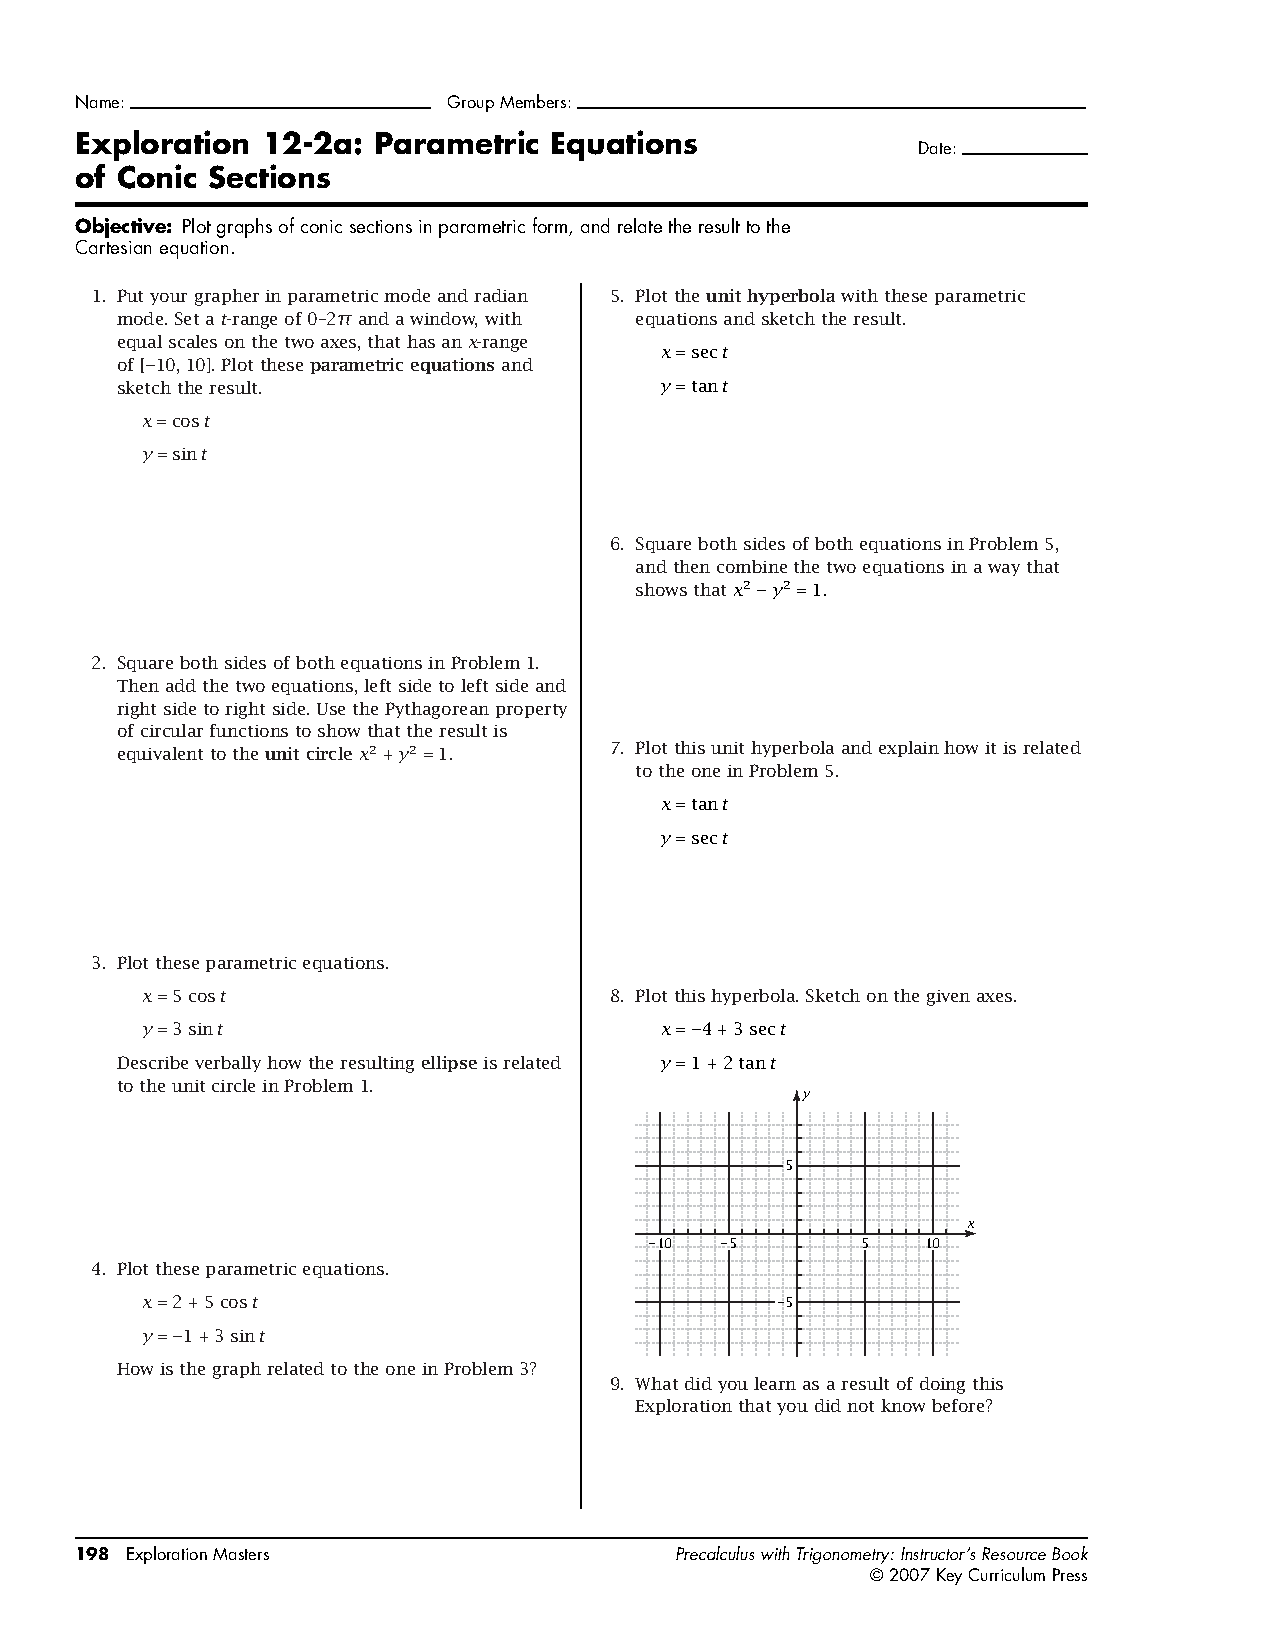
\includegraphics[width=\paperwidth]{chDD/DD02p.pdf}}
\subsection{Parametric Forms}
Conic sections lend themselves incredibly well to a variety of forms.  We saw in the last 
section that the Cartesian forms used for graphing are very versatile, always showing
a center $(h,k)$, as well as some other feature(s).  These attributes are all preserved when
we switch from graphing a relation with $x$ and $y$, to a set of functions with $x$ and $y$
both in terms of $t$.  

\begin{derivation}{Parametric Equations Ellipses}
\begin{equation}
	\begin{cases}
	x = a\sin(t) + h \\
	y = b\sin(t) + k\\
	\end{cases}
	\quad \text{or} \quad
	\begin{cases}
	x = b\sin(t) + h \\
	y = a\sin(t) + k\\
	\end{cases}
\end{equation}
\end{derivation}

As we saw in the Lab, these forms are completely interchangeable with the Cartesian equations,
by the Pythagorean Trigonometric Identities.  Because one is the sum of squares, and the other two
are the difference of squares, the latter are completely identical, but, as a rule, we only every use
tangent and secant.

\begin{derivation}{Parametric Equations of Hyperbolas}
\begin{equation}
	\begin{cases}
	x = a\sec(t) + h\\
	y = b\tan(t) + k\\
	\end{cases}
	\quad \text{or} \quad
	\begin{cases}
	x = b\tan{t} + h\\
	y = a\sec(t) + k\\
	\end{cases}
\end{equation}
\end{derivation}

\subsection{Algebra General Form}
The unity of conics sections is deep and wide.  Not only do they have a common geometric
origin, but they also all share the same algebraic origin, as the next order of general equations
after lines.  You will recall that there is a general form of linear equations, $Ax + By + C = 0$.
The general form of quadratic equations is similar: $Ax^2 + Bxy + Cy^2 + Dx + Ey + F=0$.

\subsubsection{Using a Calculator}
These conic sections are not functions (having multiple outputs per input), but only just.
There are never more than two $y$ values for any $x$ input, so they can be graphed on
your TI-8* by entering two equations.  To do that, we need to solve for $y$ first.

While there are two variable present in these equations, we are only interested in one of them
at a time, so we may regard the general form as a quadratic in $y$ with difficult coefficients:

\begin{equation*}
(C)y^2 + (Bx + E)y + (Ax^2  + Dx + F) = 0
\end{equation*}

By application of the Quadratic Formula, we can produce two equations for $y$:

\begin{equation}
y = \frac{-Bx - E \pm \sqrt{(Bx + E)^2 - 4\cdot{}C(Ax^2 + Dx + F)}}{2C}
\end{equation}

\subsubsection{Discriminant}
The presence of a $B$ term makes a conic \emph{much} more complicated, namely by 
rotating it.  We will consider rotation in the next section, but there is a formula which
applies to conics --- no matter how complicated --- to determine their classification.
To understand where it comes from, consider that only $A$, $B$, and $C$ contribute
to the overall shape (differing from the general linear form).  If we divide
$Ax^2 + Bxy + Cy^2 = 0$ by $x^2$, we see that it is a quadratic in $\left(\frac{y}{x}\right)$.
The number of solution to that equation dictates what shape the graph will be.
\begin{enumerate}
\item If $B^2 - 4AC > 0$, then it is a hyperbola.
\item If $B^2 - 4AC = 0$, then it is a parabola.
\item If $B^2 - 4AC < 0$, then it is a eclipse.
\end{enumerate}



\newpage
\section{Rotated Conics}
\subsection{Cartesian Rotation Equations}

\subsection{Parametric Rotation by Matrix}
As we saw in §B.1, there exists a simple linear transformation to rotate any $2\times 1$ 
matrix by angle $\theta$:
\begin{equation*}
\begin{bmatrix}
	\cos\theta & -\sin\theta \\
	\sin\theta & \cos\theta \\
\end{bmatrix}
\end{equation*}

\begin{example}
\exProblem
Rotate the parametric equations $x=\sec{t}, y=\tan{t}$ by $\frac{\tau}{8}$, simplify, and convert to
Cartesian.

\exSolution
We begin with the given equations, 
$$
\begin{bmatrix} x \\ y \end{bmatrix}
=
\begin{bmatrix} \sec{t} \\ \tan{t} \end{bmatrix}
$$
and left-multiply by
$$
\begin{bmatrix} \cos\frac{\tau}{8} & -\sin\frac{\tau}{8} \\
\sin\frac{\tau}{8} & \cos\frac{\tau}{8} \end{bmatrix}
=
\begin{bmatrix} \frac{\sqrt{2}}{2} & -\frac{\sqrt{2}}{2} \\
\frac{\sqrt{2}}{2} & \frac{\sqrt{2}}{2} \end{bmatrix}
$$
which gives us 
$$
\begin{bmatrix} x \\ y \end{bmatrix}
=
\begin{bmatrix}
\frac{\sqrt{2}}{2}\sec{t} - \frac{\sqrt{2}}{2}\tan{t} \\
\frac{\sqrt{2}}{2}\sec{t} + \frac{\sqrt{2}}{2}\tan{t}
\end{bmatrix}
$$
This requires some strategic thinking on our part.  Adding or subtracting the equations would can
a term, but not yield anything which could be further reduced.  \emph{Multiplying} them, however,
produces a difference of trigonometric squares, which is precisely the identity we are hoping to use.
This means $xy = \frac{2}{4}\sec^2{t} - \frac{2}{4}\tan^2{t}$.  By factoring out the half, we can use
the identity $\sec^2{t}-\tan^2{t}=1$, and get that $xy=\frac{1}{2}$.
\end{example}


\newpage
\section{Eccentricity}
\subsection{Foci}
For simplicity's sake, let us consider conics about the origin.  The circle is clearly a special case,
``the set of all points a constant distance (the \textbf{radius}) from the center.''  As we consider how to 
build an ellipse, it can be sketched as ``the set of all points who sum of their distances from 
two points (called the \textbf{foci} --- the plural of \textbf{focus}) is a constant.''

Now, we can clearly move the foci and yet keep the long-ends of an ellipse in place.  This
suggest comparing the ratio of the distance from the center to the foci ($c$), to the distance
from the center to the longer edge ($a$).  This ratio is called the conics \textbf{eccentricity}.
For circles, it is 0.  For ellipses, it is in the range $(0,1)$.  At 1, the focus is on top of the major
axis, and the shape is a parabola.    If we push onward, we come to the weird world of
hyperbolas, where eccentricity is $>1$.  They can be defined by foci as ``the set of all points
who difference of their distances from two points (called the \textbf{foci}) is a constant.''

\subsubsection{Formulae}
So, to summarize, circle either have no foci, or else we might regard them as both being at
the center.  Ellipses have two foci, $c$ away from the center.  To find $c$, we use the
formula:
\begin{equation}
a^2 = b^2 + c^2
\end{equation}
As we saw back in §3.2, parabolas have but one focus, and it is $4p$ units away from the
vertex/center.  Hyperbola also have the foci inside their curves, but for them, $c$ is the
greatest length, following the formula
\begin{equation}
a^2 + b^2 = c^2
\end{equation}

\subsection{Directrices}
There is one other feature of conics we have yet to discuss, but which was mentioned back
in §3.2: a directrix.  You recall that we can also define a parabola as ``the set of all points
who distance from a point (the focus) and a line (the directrix) is a constant.''  Does such a line
exist for the other conics?  Indeed it does, and it can be defined by the very constant we have
already found, the eccentricity.

Every conic section may be defined as ``the set of all points who distance from a point
(a focus) equals the distance from a line (a directrix) times the eccentricity.''  This leads to
the formula for the distance from the center to the directrix/directrices ($d$) as:
\begin{equation}
d = \frac{a^2}{c}
\end{equation}

\subsection{Polar Forms}
In addition to the Cartesian and Parametric definitions of conics, there are also polar
forms.  Polar equations tend to be very neat when a particular feature (usually, but not
always the center) is at the pole, and horrific when it is not.  Polar equations of conics are
no different, and so we only use the form where a focus is at the pole.  With that constraint,
we can define the all at once as
\begin{equation}
r = \frac{ed}{1\pm e\cos\theta}
\end{equation}
and cosine could be sine.

\newpage
\section{3D Conics}
\noindent\makebox[\textwidth]{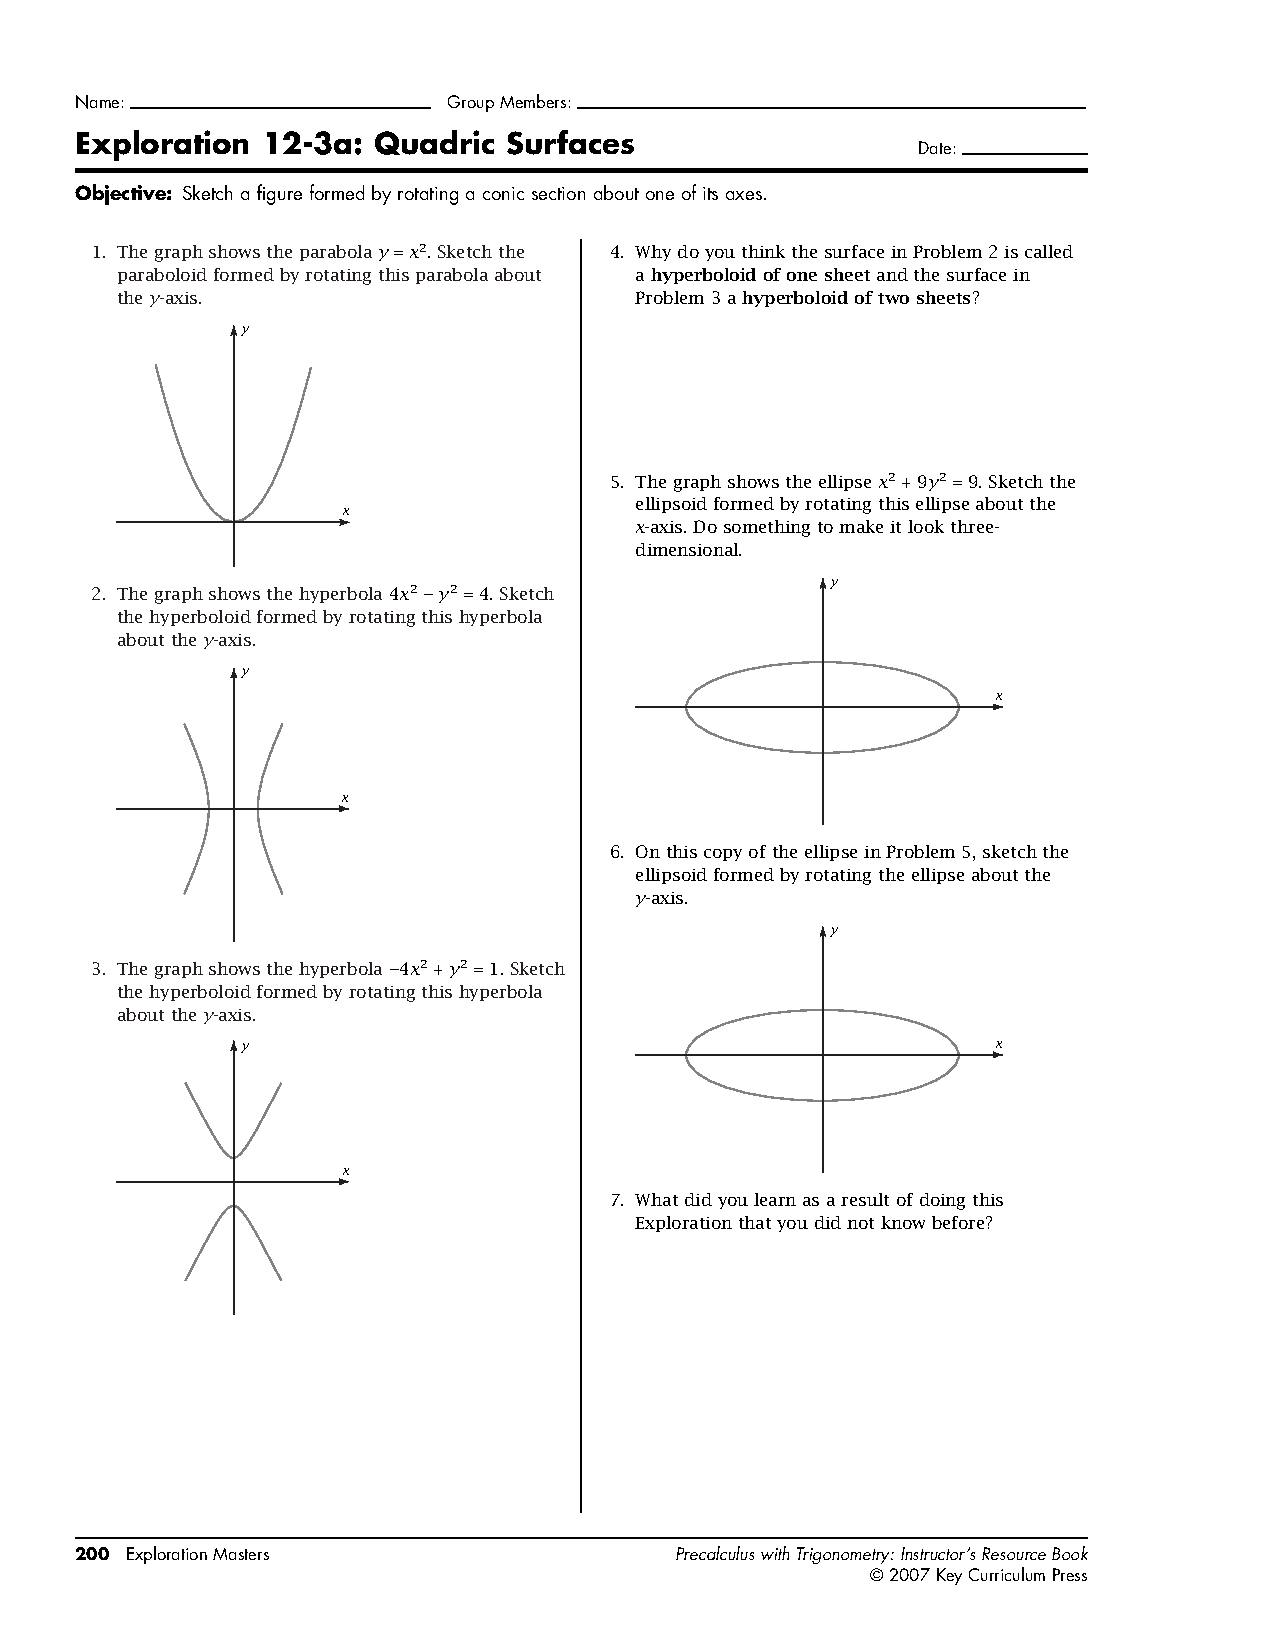
\includegraphics[width=\paperwidth]{chDD/DD05p.pdf}}
\subsection{2.5D}
\subsection{$x, y, z$}
\subsection{$r, \theta, z$}
\subsection{$\rho, \phi, \theta$}

\section{Chapter Review}